\documentclass[12pt]{article}
\usepackage[utf8]{inputenc}
\usepackage{amsmath,amsthm,amsfonts,amssymb}
\usepackage{tikz}
\usepackage{subfig}
\usepackage[english]{babel}
\usepackage{capt-of}
\newtheorem{theorem}{Theorem}
\usetikzlibrary{calc}
\usetikzlibrary{shapes}
\usepackage{hyperref}
%might be unnecessary
\usepackage{doi}

%bibliography CMDS

%\usepackage{cite}
%\usepackage[style=alphabetic]{biblatex}
%\bibliographystyle{plain}

%\usepackage[style=alphabetic]{biblatex}

\usepackage[backend=biber,style=alphabetic]{biblatex}
%\usepackage[backend=bibtex,style=alphabetic]{biblatex}
\addbibresource{bibb.bib}

%%% With amsthm package, creates environments for nicely formatted,
%%% labeled, and numbered propositions, etc.
\theoremstyle{plain}
\newtheorem{thm}{Theorem}
\newtheorem{lemma}[thm]{Lemma}
\newtheorem{prop}[thm]{Proposition}
\newtheorem{conj}[thm]{Conjecture}
\newtheorem{cor}[thm]{Corollary}
\newtheorem{claim}[thm]{Claim}
\newtheorem{fact}[thm]{Fact}

\theoremstyle{definition}
\newtheorem{eg}[thm]{Example}
\newtheorem{defn}[thm]{Definition}
\newtheorem{rem}[thm]{Remark}
\newtheorem{observ}[thm]{Observation}
\newtheorem{open}[thm]{Open Problem}
\newtheorem{prob.}[thm]{Problem}
\newtheorem{quest}[thm]{Question}

% I used these for making definitions and theorems, not what is above
\theoremstyle{remark}
\newtheorem{remark}[thm]{Remark}
\newtheorem{note}[thm]{Note}
\theoremstyle{definition}
\newtheorem{definition}{Definition}[section]
\newtheorem{exmp}{Example}[section]

%custom commands

% blank cell
\newcommand{\cell}[4]{ \draw[thick] ( #1 , #2 ) rectangle ( #3 , #4 );}

% open cell 
\newcommand{\cellopen}[4]{ \draw[thick] ( #1 , #2 ) rectangle ( #3 , #4 ); \node[shape=circle,draw=red,fill=red, inner sep=0pt,minimum size=3pt] (A) at ( #1 * 0.5 + #3 * 0.5 , #2 * 0.5 + #4 * 0.5 ){};}

% /
\newcommand{\cellA}[4]{ \draw[thick] ( #1 , #2 ) rectangle ( #3 , #4 ); \draw[red, thick] (#3 * 0.5 + #1 * 0.5 , #2) -- (#3, #4 * 0.5 + #2 * 0.5);}

% \
\newcommand{\cellB}[4]{ \draw[thick] ( #1 , #2 ) rectangle ( #3 , #4 ); \draw[red, thick] (#3 * 0.5 + #1 * 0.5 , #2) -- (#1, #4 * 0.5 + #2 * 0.5);}

% /
\newcommand{\cellC}[4]{ \draw[thick] ( #1 , #2 ) rectangle ( #3 , #4 ); \draw[red, thick] (#3 * 0.5 + #1 * 0.5 , #4) -- (#1, #4 * 0.5 + #2 * 0.5);}

% L
\newcommand{\cellD}[4]{ \draw[thick] ( #1 , #2 ) rectangle ( #3 , #4 ); \draw[red, thick] (#3 * 0.5 + #1 * 0.5 , #4) -- (#3, #4 * 0.5 + #2 * 0.5);}

% |
\newcommand{\cellE}[4]{ \draw[thick] ( #1 , #2 ) rectangle ( #3 , #4 ); \draw[red, thick] (#3 * 0.5 + #1 * 0.5 , #2) -- (#3 * 0.5 + #1 * 0.5 , #4);}

% -
\newcommand{\cellF}[4]{ \draw[thick] ( #1 , #2 ) rectangle ( #3 , #4 ); \draw[red, thick] (#3, #4 * 0.5 + #2 * 0.5) -- (#1, #4 * 0.5 + #2 * 0.5);}

\newcommand{\cellAf}[4]{\filldraw[gray!40] ( #1 , #2 ) rectangle ( #3 , #4 ); \draw[thick] ( #1 , #2 ) rectangle ( #3 , #4 ); \draw[red, thick] (#3 * 0.5 + #1 * 0.5 , #2) -- (#3, #4 * 0.5 + #2 * 0.5);}

% \
\newcommand{\cellBf}[4]{\filldraw[gray!40] ( #1 , #2 ) rectangle ( #3 , #4 ); \draw[thick] ( #1 , #2 ) rectangle ( #3 , #4 ); \draw[red, thick] (#3 * 0.5 + #1 * 0.5 , #2) -- (#1, #4 * 0.5 + #2 * 0.5);}

% /
\newcommand{\cellCf}[4]{\filldraw[gray!40] ( #1 , #2 ) rectangle ( #3 , #4 ); \draw[thick] ( #1 , #2 ) rectangle ( #3 , #4 ); \draw[red, thick] (#3 * 0.5 + #1 * 0.5 , #4) -- (#1, #4 * 0.5 + #2 * 0.5);}

% L
\newcommand{\cellDf}[4]{\filldraw[gray!40] ( #1 , #2 ) rectangle ( #3 , #4 ); \draw[thick] ( #1 , #2 ) rectangle ( #3 , #4 ); \draw[red, thick] (#3 * 0.5 + #1 * 0.5 , #4) -- (#3, #4 * 0.5 + #2 * 0.5);}

% |
\newcommand{\cellEf}[4]{\filldraw[gray!40] ( #1 , #2 ) rectangle ( #3 , #4 ); \draw[thick] ( #1 , #2 ) rectangle ( #3 , #4 ); \draw[red, thick] (#3 * 0.5 + #1 * 0.5 , #2) -- (#3 * 0.5 + #1 * 0.5 , #4);}

% -
\newcommand{\cellFf}[4]{\filldraw[gray!40] ( #1 , #2 ) rectangle ( #3 , #4 ); \draw[thick] ( #1 , #2 ) rectangle ( #3 , #4 ); \draw[red, thick] (#3, #4 * 0.5 + #2 * 0.5) -- (#1, #4 * 0.5 + #2 * 0.5);}


\newcommand{\lablnode}[3]{\node[shape=circle,draw=white,fill=white, inner sep=0pt,minimum size=1pt] (A) at ( #1 , #2 ) {#3};}

\usepackage[margin=1in]{geometry}

%doc info
\title{Mosaics}
\author{Jack Hanke, Farstar31}
\date{\today}

\begin{document}

\begin{center}
    \Large
    \textbf{Mosaics}
    
    \vspace{0.4cm}
    \large
    
    Jack Hanke   
    \vspace{0.4cm}
    
    \today
    \vspace{0.4cm}    
\end{center}

\section{Introduction}

Consider the following $6$ unit squares with markings on them.

%figure of tiles (colored marknigs!)
\begin{center}
    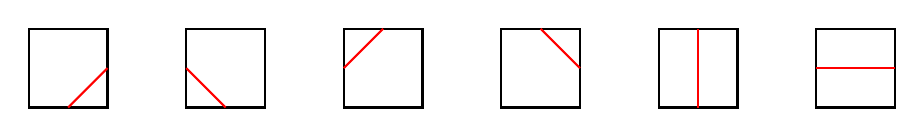
\begin{tikzpicture}
    \cellA{0}{0}{1}{1}
    \cellB{2}{0}{3}{1}
    \cellC{4}{0}{5}{1}
    \cellD{6}{0}{7}{1}
    \cellE{8}{0}{9}{1}
    \cellF{10}{0}{11}{1}    
    \end{tikzpicture}
\end{center}

Call these squares \textit{tiles}. 

\begin{definition}
An $(n,m)$-\textit{mosaic} is a rectangular grid made up of tiles.
\end{definition}

\begin{exmp}
An example of a $(7,5)$-mosaic:
\begin{center}
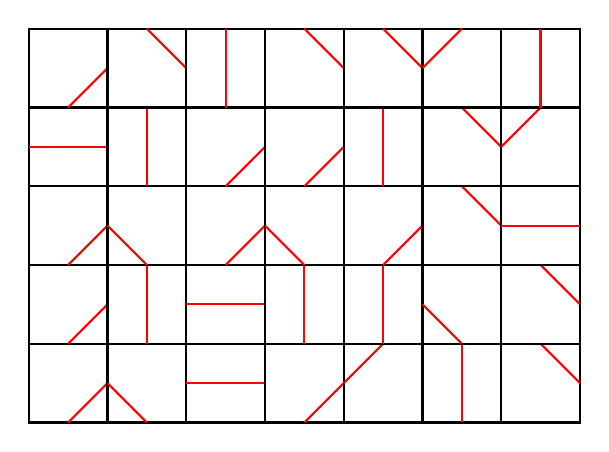
\begin{tikzpicture}
    % row1
    \cellA{0}{0}{1}{1}
    \cellB{1}{0}{2}{1}
    \cellF{2}{0}{3}{1}
    \cellA{3}{0}{4}{1}
    \cellC{4}{0}{5}{1}
    \cellE{5}{0}{6}{1}
    \cellD{6}{0}{7}{1}
    % row2
    \cellA{0}{1}{1}{2}
    \cellE{1}{1}{2}{2}
    \cellF{2}{1}{3}{2}
    \cellE{3}{1}{4}{2}
    \cellE{4}{1}{5}{2}
    \cellB{5}{1}{6}{2}
    \cellD{6}{1}{7}{2}
    % row3
    \cellA{0}{2}{1}{3}
    \cellB{1}{2}{2}{3}
    \cellA{2}{2}{3}{3}
    \cellB{3}{2}{4}{3}
    \cellA{4}{2}{5}{3}
    \cellD{5}{2}{6}{3}
    \cellF{6}{2}{7}{3}
    % row4
    \cellF{0}{3}{1}{4}
    \cellE{1}{3}{2}{4}
    \cellA{2}{3}{3}{4}
    \cellA{3}{3}{4}{4}
    \cellE{4}{3}{5}{4}
    \cellD{5}{3}{6}{4}
    \cellC{6}{3}{7}{4}
    % row5
    \cellA{0}{4}{1}{5}
    \cellD{1}{4}{2}{5}
    \cellE{2}{4}{3}{5}
    \cellD{3}{4}{4}{5}
    \cellD{4}{4}{5}{5}
    \cellC{5}{4}{6}{5}
    \cellE{6}{4}{7}{5}
\end{tikzpicture}
\end{center}
\end{exmp}

Clearly there are $6^{nm}$ possible mosaics. Which of these mosaics contain self-avoiding polygons?

%example of a mosaic with an enclosed region
\begin{exmp}
\label{exp:sap}
An example of a $(7,5)$-mosaic with a self-avoiding polygon, hilighted in gray:
\begin{center}
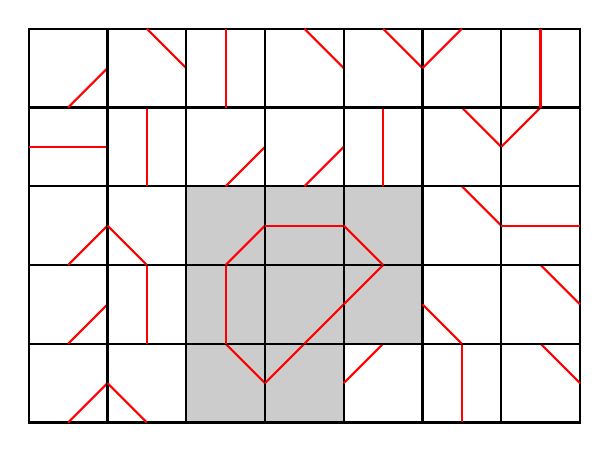
\begin{tikzpicture}
    % row1
    \cellA{0}{0}{1}{1}
    \cellB{1}{0}{2}{1}
    \cellDf{2}{0}{3}{1}
    \cellCf{3}{0}{4}{1}
    \cellC{4}{0}{5}{1}
    \cellE{5}{0}{6}{1}
    \cellD{6}{0}{7}{1}
    % row2
    \cellA{0}{1}{1}{2}
    \cellE{1}{1}{2}{2}
    \cellEf{2}{1}{3}{2}
    \cellAf{3}{1}{4}{2}
    \cellCf{4}{1}{5}{2}
    \cellB{5}{1}{6}{2}
    \cellD{6}{1}{7}{2}
    % row3
    \cellA{0}{2}{1}{3}
    \cellB{1}{2}{2}{3}
    \cellAf{2}{2}{3}{3}
    \cellFf{3}{2}{4}{3}
    \cellBf{4}{2}{5}{3}
    \cellD{5}{2}{6}{3}
    \cellF{6}{2}{7}{3}
    % row4
    \cellF{0}{3}{1}{4}
    \cellE{1}{3}{2}{4}
    \cellA{2}{3}{3}{4}
    \cellA{3}{3}{4}{4}
    \cellE{4}{3}{5}{4}
    \cellD{5}{3}{6}{4}
    \cellC{6}{3}{7}{4}
    % row5
    \cellA{0}{4}{1}{5}
    \cellD{1}{4}{2}{5}
    \cellE{2}{4}{3}{5}
    \cellD{3}{4}{4}{5}
    \cellD{4}{4}{5}{5}
    \cellC{5}{4}{6}{5}
    \cellE{6}{4}{7}{5}
\end{tikzpicture}
\end{center}
\end{exmp}

Let $t_{n,m}$ be the number of mosaics that have at least one self avoiding polygon (SAP). From the fact that the smallest SAP is

\begin{center}
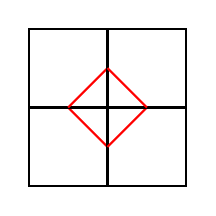
\begin{tikzpicture}
% row1
\cellD{0}{0}{1}{1}
\cellC{1}{0}{2}{1}
% row2
\cellA{0}{1}{1}{2}
\cellB{1}{1}{2}{2}
\end{tikzpicture}
\end{center}

we have that $t_{n,1}=t_{1,m}=0$, and $t_{2,2} = 1$. What else can be said?

\begin{thm}

TODO finish theorem writeup

$$
M(2) = \begin{bmatrix}
36 & 1 \\
-1 & 1
\end{bmatrix}
$$

For $h \geq 2$, then if
$$
M(h) = \begin{bmatrix}
M_1 & M_2 \\
M_3 & M_4
\end{bmatrix}
$$

then
$$
M(h+1) = \begin{bmatrix}
6M_1 & 6M_2 & \frac{1}{6}M_1 & 1M_2 \\
6M_3 & 6M_4 & 0M_3 & 1M_4 \\
-\frac{1}{6}M_1 & 0M_2 & \frac{1}{6}M_1 & 1M_2 \\
1M_3 & 1M_4 & -1M_3 & 6M_4 \\
\end{bmatrix}
$$

where $M_i$ is a sub-matrix (or possible a scalar) of the block matrix $M$.    

Then $t_{n,m}=?$

\end{thm}

\begin{proof}
Begin by labelling the vertices of the rectangular lattice as follows. If the vertex is surrounded by an even number of SAPs, color it black. If the vertex is surrounded by an odd number of SAPs, color it green. Using the diagram from Example \ref{exp:sap} above, we get the following labelling. Notice that vertices on the boundary of the lattice will always be black.

\begin{center}
    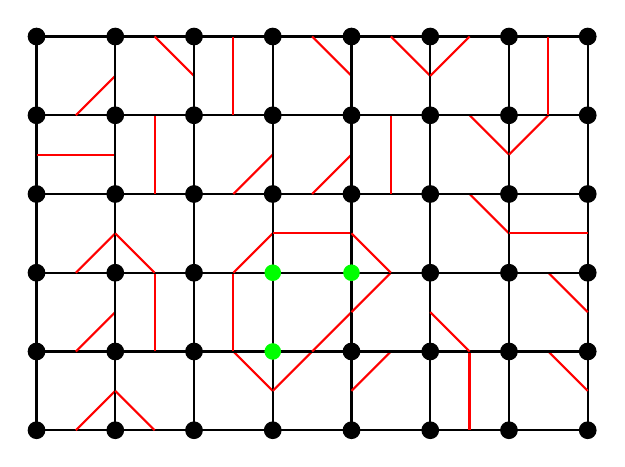
\begin{tikzpicture}
        % row1
        \cellA{0}{0}{1}{1}
        \cellB{1}{0}{2}{1}
        \cellD{2}{0}{3}{1}
        \cellC{3}{0}{4}{1}
        \cellC{4}{0}{5}{1}
        \cellE{5}{0}{6}{1}
        \cellD{6}{0}{7}{1}
        % row2
        \cellA{0}{1}{1}{2}
        \cellE{1}{1}{2}{2}
        \cellE{2}{1}{3}{2}
        \cellA{3}{1}{4}{2}
        \cellC{4}{1}{5}{2}
        \cellB{5}{1}{6}{2}
        \cellD{6}{1}{7}{2}
        % row3
        \cellA{0}{2}{1}{3}
        \cellB{1}{2}{2}{3}
        \cellA{2}{2}{3}{3}
        \cellF{3}{2}{4}{3}
        \cellB{4}{2}{5}{3}
        \cellD{5}{2}{6}{3}
        \cellF{6}{2}{7}{3}
        % row4
        \cellF{0}{3}{1}{4}
        \cellE{1}{3}{2}{4}
        \cellA{2}{3}{3}{4}
        \cellA{3}{3}{4}{4}
        \cellE{4}{3}{5}{4}
        \cellD{5}{3}{6}{4}
        \cellC{6}{3}{7}{4}
        % row5
        \cellA{0}{4}{1}{5}
        \cellD{1}{4}{2}{5}
        \cellE{2}{4}{3}{5}
        \cellD{3}{4}{4}{5}
        \cellD{4}{4}{5}{5}
        \cellC{5}{4}{6}{5}
        \cellE{6}{4}{7}{5}
        % label for row1
        \draw[fill=black] (0,0) circle (3pt);
        \draw[fill=black] (1,0) circle (3pt);
        \draw[fill=black] (2,0) circle (3pt);
        \draw[fill=black] (3,0) circle (3pt);
        \draw[fill=black] (4,0) circle (3pt);
        \draw[fill=black] (5,0) circle (3pt);
        \draw[fill=black] (6,0) circle (3pt);
        \draw[fill=black] (7,0) circle (3pt);
        % label for row1
        \draw[fill=black] (0,1) circle (3pt);
        \draw[fill=black] (1,1) circle (3pt);
        \draw[fill=black] (2,1) circle (3pt);
        \draw[fill=green, draw=none] (3,1) circle (3pt);
        \draw[fill=black] (4,1) circle (3pt);
        \draw[fill=black] (5,1) circle (3pt);
        \draw[fill=black] (6,1) circle (3pt);
        \draw[fill=black] (7,1) circle (3pt);
        % label for row1
        \draw[fill=black] (0,2) circle (3pt);
        \draw[fill=black] (1,2) circle (3pt);
        \draw[fill=black] (2,2) circle (3pt);
        \draw[fill=green, draw=none] (3,2) circle (3pt);
        \draw[fill=green, draw=none] (4,2) circle (3pt);
        \draw[fill=black] (5,2) circle (3pt);
        \draw[fill=black] (6,2) circle (3pt);
        \draw[fill=black] (7,2) circle (3pt);
        % label for row1
        \draw[fill=black] (0,3) circle (3pt);
        \draw[fill=black] (1,3) circle (3pt);
        \draw[fill=black] (2,3) circle (3pt);
        \draw[fill=black] (3,3) circle (3pt);
        \draw[fill=black] (4,3) circle (3pt);
        \draw[fill=black] (5,3) circle (3pt);
        \draw[fill=black] (6,3) circle (3pt);
        \draw[fill=black] (7,3) circle (3pt);
        % label for row1
        \draw[fill=black] (0,4) circle (3pt);
        \draw[fill=black] (1,4) circle (3pt);
        \draw[fill=black] (2,4) circle (3pt);
        \draw[fill=black] (3,4) circle (3pt);
        \draw[fill=black] (4,4) circle (3pt);
        \draw[fill=black] (5,4) circle (3pt);
        \draw[fill=black] (6,4) circle (3pt);
        \draw[fill=black] (7,4) circle (3pt);
        % label for row1
        \draw[fill=black] (0,5) circle (3pt);
        \draw[fill=black] (1,5) circle (3pt);
        \draw[fill=black] (2,5) circle (3pt);
        \draw[fill=black] (3,5) circle (3pt);
        \draw[fill=black] (4,5) circle (3pt);
        \draw[fill=black] (5,5) circle (3pt);
        \draw[fill=black] (6,5) circle (3pt);
        \draw[fill=black] (7,5) circle (3pt);
    \end{tikzpicture}
\end{center}

Considering an individual cell, with the four associated labels.  We call the surrounding vertice labels the cell's \textit{parity}. The $16$ possible parities, along with their associated weight, are shown in the following diagram.

\begin{center}
    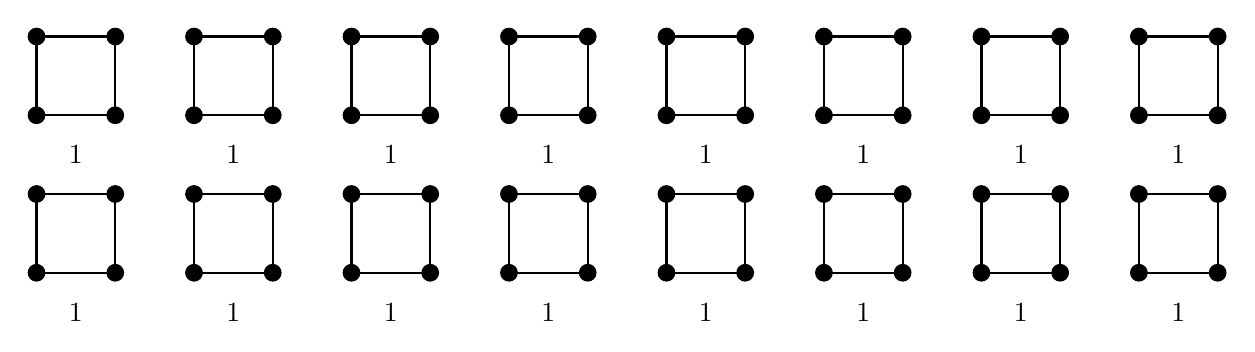
\begin{tikzpicture}
        % row1
        \cell{0}{0}{1}{1}
        \cell{2}{0}{3}{1}
        \cell{4}{0}{5}{1}
        \cell{6}{0}{7}{1}
        \cell{8}{0}{9}{1}
        \cell{10}{0}{11}{1}
        \cell{12}{0}{13}{1}
        \cell{14}{0}{15}{1}
        % row2
        \cell{0}{2}{1}{3}
        \cell{2}{2}{3}{3}
        \cell{4}{2}{5}{3}
        \cell{6}{2}{7}{3}
        \cell{8}{2}{9}{3}
        \cell{10}{2}{11}{3}
        \cell{12}{2}{13}{3}
        \cell{14}{2}{15}{3}
        % label for row1
        \draw[fill=black] (0,0) circle (3pt);
        \draw[fill=black] (1,0) circle (3pt);
        \draw[fill=black] (2,0) circle (3pt);
        \draw[fill=black] (3,0) circle (3pt);
        \draw[fill=black] (4,0) circle (3pt);
        \draw[fill=black] (5,0) circle (3pt);
        \draw[fill=black] (6,0) circle (3pt);
        \draw[fill=black] (7,0) circle (3pt);
        \draw[fill=black] (8,0) circle (3pt);
        \draw[fill=black] (9,0) circle (3pt);
        \draw[fill=black] (10,0) circle (3pt);
        \draw[fill=black] (11,0) circle (3pt);
        \draw[fill=black] (12,0) circle (3pt);
        \draw[fill=black] (13,0) circle (3pt);
        \draw[fill=black] (14,0) circle (3pt);
        \draw[fill=black] (15,0) circle (3pt);
        % label for row1
        \draw[fill=black] (0,1) circle (3pt);
        \draw[fill=black] (1,1) circle (3pt);
        \draw[fill=black] (2,1) circle (3pt);
        \draw[fill=black] (3,1) circle (3pt);
        \draw[fill=black] (4,1) circle (3pt);
        \draw[fill=black] (5,1) circle (3pt);
        \draw[fill=black] (6,1) circle (3pt);
        \draw[fill=black] (7,1) circle (3pt);
        \draw[fill=black] (8,1) circle (3pt);
        \draw[fill=black] (9,1) circle (3pt);
        \draw[fill=black] (10,1) circle (3pt);
        \draw[fill=black] (11,1) circle (3pt);
        \draw[fill=black] (12,1) circle (3pt);
        \draw[fill=black] (13,1) circle (3pt);
        \draw[fill=black] (14,1) circle (3pt);
        \draw[fill=black] (15,1) circle (3pt);
        % label for row1
        \draw[fill=black] (0,2) circle (3pt);
        \draw[fill=black] (1,2) circle (3pt);
        \draw[fill=black] (2,2) circle (3pt);
        \draw[fill=black] (3,2) circle (3pt);
        \draw[fill=black] (4,2) circle (3pt);
        \draw[fill=black] (5,2) circle (3pt);
        \draw[fill=black] (6,2) circle (3pt);
        \draw[fill=black] (7,2) circle (3pt);
        \draw[fill=black] (8,2) circle (3pt);
        \draw[fill=black] (9,2) circle (3pt);
        \draw[fill=black] (10,2) circle (3pt);
        \draw[fill=black] (11,2) circle (3pt);
        \draw[fill=black] (12,2) circle (3pt);
        \draw[fill=black] (13,2) circle (3pt);
        \draw[fill=black] (14,2) circle (3pt);
        \draw[fill=black] (15,2) circle (3pt);
        % label for row1
        \draw[fill=black] (0,3) circle (3pt);
        \draw[fill=black] (1,3) circle (3pt);
        \draw[fill=black] (2,3) circle (3pt);
        \draw[fill=black] (3,3) circle (3pt);
        \draw[fill=black] (4,3) circle (3pt);
        \draw[fill=black] (5,3) circle (3pt);
        \draw[fill=black] (6,3) circle (3pt);
        \draw[fill=black] (7,3) circle (3pt);
        \draw[fill=black] (8,3) circle (3pt);
        \draw[fill=black] (9,3) circle (3pt);
        \draw[fill=black] (10,3) circle (3pt);
        \draw[fill=black] (11,3) circle (3pt);
        \draw[fill=black] (12,3) circle (3pt);
        \draw[fill=black] (13,3) circle (3pt);
        \draw[fill=black] (14,3) circle (3pt);
        \draw[fill=black] (15,3) circle (3pt);
        % numbers row 1
        \( \lablnode{0.5}{-0.5}{1} \)
        \( \lablnode{2.5}{-0.5}{1} \)
        \( \lablnode{4.5}{-0.5}{1} \)
        \( \lablnode{6.5}{-0.5}{1} \)
        \( \lablnode{8.5}{-0.5}{1} \)
        \( \lablnode{10.5}{-0.5}{1} \)
        \( \lablnode{12.5}{-0.5}{1} \)
        \( \lablnode{14.5}{-0.5}{1} \)
        % numbers row 2
        \( \lablnode{0.5}{1.5}{1} \)
        \( \lablnode{2.5}{1.5}{1} \)
        \( \lablnode{4.5}{1.5}{1} \)
        \( \lablnode{6.5}{1.5}{1} \)
        \( \lablnode{8.5}{1.5}{1} \)
        \( \lablnode{10.5}{1.5}{1} \)
        \( \lablnode{12.5}{1.5}{1} \)
        \( \lablnode{14.5}{1.5}{1} \)
    \end{tikzpicture}
\end{center}

TODO complete proof writeup

\end{proof}

\end{document}